(γ) Αν ο $\left(X,\langle\cdot,\cdot\rangle\right)$ είναι χώρος \tl{Hilbert} 
(δηλαδή, ο $X$ είναι χώρος με εσωτερικό γινόμενο, ο οποίος είναι χώρος 
\tl{Banach} με τη νόρμα που επάγεται από το $\langle\cdot,\cdot\rangle$), τότε η
απεικόνιση
\begin{equation*}
    \langle\cdot,\cdot\rangle : L_2\left([a,\infty],X\right)^2 \rightarrow 
    \realf\quad\text{με}\quad \langle f, g \rangle = \int_o^{\infty}\langle f(t)
    ,g(t) \rangle
\end{equation*}
είναι εσωτερικό γινόμενο στο $L_2([a,\infty],X):$ Από την ανισότητα \tl{Cauchy-
Schwarz} και την πρώτη ανισότητα που αποδείχθηκε στο (β), προκύπτει όροι
\begin{equation*}
    \int_a^{\infty}\langle f(t),g(t) \rangle \leq \int_a^{\infty} ||f(t)||\,
    ||g(t)|| \leq ||f(t)||\,||g(t)|| \leq \infty.    
\end{equation*}
H θετικότητα της $\langle\cdot,\cdot\rangle$ έχει αποδειχθεί στο (β). Οι 
υπόλοιπες ιδιότητες (διγραμμικότητα, συμμετρία) είναι προφανείς.

Σχόλια: οι χώροι $L_2\left([a,\infty],X\right)$ δεν είναι εν γένει χώρος 
\tl{Banach} (δηλαδή δεν είναι απαραίτητα πλήρης). Πολλά προβλήματα στη θεωρία 
ελέγχου γραμμικών συστημάτων, βασίζονται στην επίλυση γραμμικών τετραγωνικών 
προβλημάτων βελτίστου ελέγχου. Τα προβλήματα αυτά μπορούν να διατυπωθούν ως 
προβλήματα ελαχίστης νόρμας, τα οποία μπορούν να αντιμετωπιστούν αποτελεσματικά
με το θεώρημα προβολής σε χώρους \tl{Hilbert}.

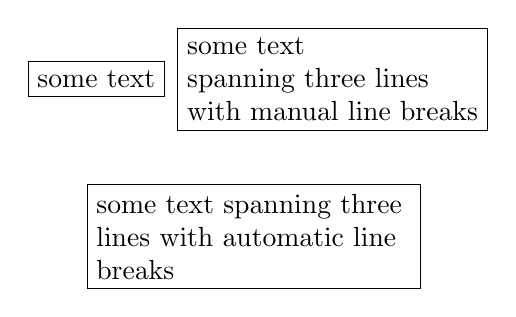
\begin{tikzpicture}
    \node[draw] at (0,0) {some text};
    \node[draw,align=left] at (3,0) {some text\\ spanning three lines\\ with manual line breaks};
    \node[draw,text width=4cm] at (2,-2) {some text spanning three lines with automatic line breaks};
\end{tikzpicture}